\section{The Signum! word processor}

The \gls{Signum!2} word processor is a computer program written by Franz Schmerbeck\footnote{\url{http://schmerbeck.de/}} for the ATARI ST in the 1980s. It was and still is being distributed by the Heidelberg-based company \gls{ASH} (ASH), which has also provided user-support. ASH furthermore published a comprehensive guide in book form \cite{ritzhaupt1988signum}.

In his foreword to \textit{Das Signum! Buch}, the author of \Signum{} explains that the program was written for all the users who were limited by the \textquote{Standard of normal word processing systems}. He ended up writing his own thesis for a mathematics degree (\textit{Diplom}) on a typewriter for lack of alternatives and explains:

\foreignblockquote{german}[{\cite[Page 7]{ritzhaupt1988signum}}]{
    %Die Idee zur Entwicklung von Signum entspringt eigenen (mühsamen) Erfahrungen im Bereich der Textverarbeitung. Sie gipfelte in der Erstellung einer Diplomarbeit in Mathematik mit einer Schreibmaschine. Jeder, der eine solche Arbeit einmal gesehen hat, weiß, was das bedeutet: Griechische Symbole und mathematische Sonderzeichen kommen fast mit der selben Häufigkeit vor wie normaler Fließtext. Dies bedeutet ein ständiges Wechseln zwischen mindestens drei verschiedenen Kugelköpfen.
    
    Tritt man aus dem Elfenbeinturm der eigenen Fakultät, so erkennt man, daß viele Textanwendungen außerhalb der Naturwissenschaften mit ähnlichen Problemen behaftet sind: Man denke z.B. an mehrsprachige Übersetzungen (griechisch, kyrillisch, hebräisch), Dokumentationen im Handel, in der Technik (grafische Sonderzeichen), oder an die anspruchsvolle Aufbereitung eines Textes (verschiedene Schriftarten und -größen). Diese Anwendungen können mit Standardsysteme oft nicht oder nur mit unzureichender Qualität bewältigt werden.
    
}

These requirements are directly reflected in the implementation of \Signum{}: Firstly, its free-form layout mode allows mathematical formulas to be typeset with minimal effort and a \acrshort{wysiwyg} user interface.

Secondly, it allows the use of up to $7$ \textit{character sets} or \glspl{charset}, which are sets of 127 glyphs that are mapped to keys on the keyboard. In the editor, a user can set one charset as the default (``\textit{Normal}''), one charset to be used while holding the \textit{Alternate} key and one charset to be used while holding the \textit{Control} key.

In addition to using \glspl{charset} to have the same font in multiple sizes, this system allows the users to add text in other writing systems such as Hebrew, Arabic or Greek or simple drawings like chemical formulas, box drawing characters, smileys with minimal overhead\funfact{There's even a charset with a \textit{cut this paper here} mark.}.

The character sets also play a crucial role in making Signum! a tool that can produce high-resolution documents while using a low-resolution graphical interface. For every device that needs to display or print these characters there is a different font file. The editor uses the low-resolution \textbf{.E24} file format while a 24-needle printer would use \textbf{.P24} files that have about 3 times the resolution. There are additional file formats for other printer types.

\begin{figure}[h]
    \centering
    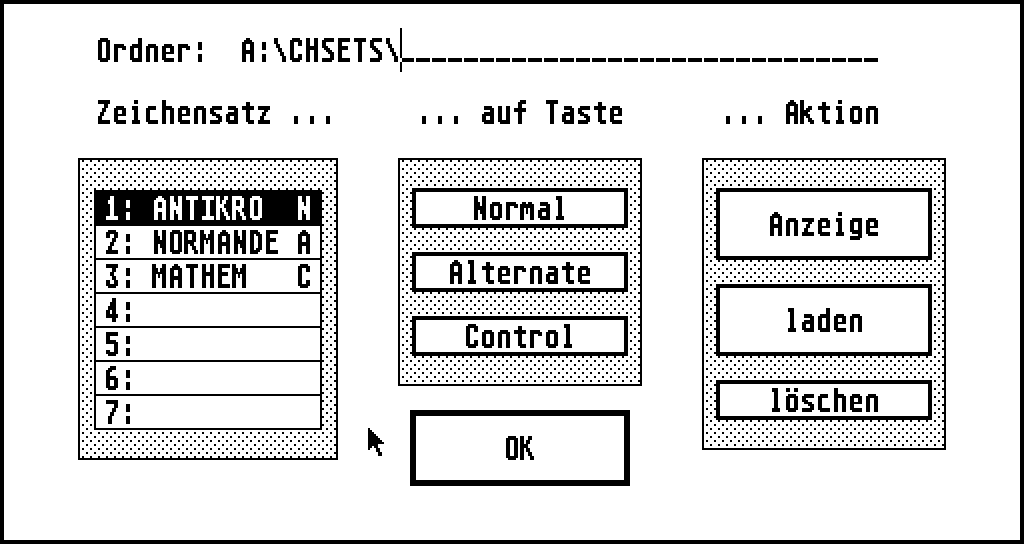
\includegraphics[width=\columnwidth]{img/cset-dialog.png}
    \caption{The character set dialog \label{fig:cset-dialog}}
\end{figure}

\subsection{Word processing with Signum!}

Given the limitations of the time, \gls{Signum!2} works very much like its modern successors. The main feature of the interface is a visual representation of a page. There is a cursor that indicates the current insertion point and when the user presses a key, the corresponding character is placed at that point and the cursor moves forward. When the cursor reaches the end of a line, it automatically moves or breaks the current word to the next line and continues from there.

A document consists of up to a hundred pages, only one of which is active at a time. The current page number is displayed in the bottom right corner of the editor. The cursor can be placed anywhere on a two by two pixel grid. The vertical component of a position in the grid is called the \textit{(micro-)line}. The value for the cursor's vertical position is also displayed in the bottom right.

There are separate header and footer areas on each page, which hold page number information and footnotes and don't interfere with breaking paragraphs across pages.

%\noindent\fixme{escape-sequences}\\
%TODO: Finally, a lot of menu commands are also available as \textit{escape-sequences}, that is sequences of key-presses that start with the \textit{escape} key. These sequences could change the position of the cursor, 

\Signum{} also has a macro system, whereby a sequence of key presses can be recorded and played back at a later point in time. This is especially useful in conjunction with the escape sequences. Escape sequences are combinations of key presses that start with \texttt{ESC} and can change settings such as the current \textit{normal} character set.

\begin{figure}
    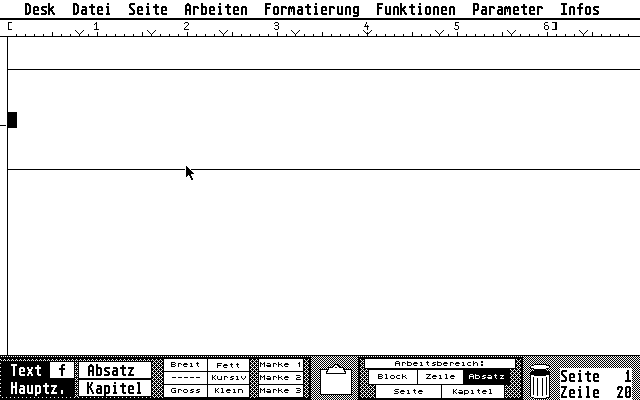
\includegraphics[width=\columnwidth]{img/SNAP3.png}
    \caption{Signum!2 immediately after starting the program. The first menu would be called \texttt{SIGNUM!} if the screenshot tool wasn't installed.}
    \label{fig:sig2_start}
\end{figure}

\subsubsection{Writing Modes}
While the grid allows for some flexibility in typesetting, the default behavior of the system guides the user to a regular page layout. In the bottom left corner of the editor, there is a set of buttons that specify the \textit{writing mode} of the current line. \textbf{Text} mode is on by default and is required for the line to be affected by formatting operations.

The writing mode for every visible line is also visualized in the column just left of the page. For example, a checkerboard pattern there means that the line is not in \textbf{Text} mode. A solid black line indicates a \textbf{Hauptz.} or main line. If not disabled in the \textit{Functions} menu, these are always set when a new line is created and correspond to the baseline of the written text.

Main lines play a special role in most operations, because all characters within \textit{index distance} of such a line are treated as the same typographical line. That means that they are moved together for operations like \textit{centering} and when the user clicks on a line within index distance of the main line, the cursor will be placed exactly on the main line, with the only exception that clinking on a character selects the position of that character, even when it's not on the main line.

The name \textit{index distance} refers to the fact that the user can press \textit{CTRL+UP/DOWN} to move the cursor by that amount, which, if used on a main line, is a simple way to create sub- and superscript that moves with the text.

The other two modes, \textbf{Absatz} (i.e. paragraph) and \textbf{Kapitel} (chapter) are used to group multiple lines so that they can be formatted as a single unit.

\subsubsection{Font Variants} \label{sec:font-variants}
The next block of buttons on the toolbar is used for modifying characters to match common font variants. They are (in editor-order, left-to-right, top-to-bottom):

\newcommand{\key}[1]{\item[{\framebox[1.2cm]{\centering #1}}]}

\begin{description}
    \key{Breit}  The width of all characters is doubled.
    \key{Fett} The characters are set in bold print.
    \key{\vphantom{U}–––––} The characters are underlined.
    \key{Kursiv} The characters are tilted $1:4$ / set in italic print.
    \key{Gross} The height of all characters is multiplied by $1.5$.
    \key{Klein} The height of all characters is multiplied by $0.75$.
\end{description}

Only \textbf{Gross} and \textbf{Klein} are mutually exclusive.

\subsubsection{Formatting}

While the system sets some sensible defaults, very little formatting is automatically applied. The \textit{automatic insertion}, that is pushing existing characters in a line to the right when typing and the \textit{automatic line feed} that is moving the cursor to the next line and pushing down existing lines are both opt-in settings in the \textbf{Funktionen} menu.

\textit{Signum!2} provides a set of text layout options in the \textbf{Arbeiten} menu. All of these are transformations that are applied to some part of the text around the cursor, depending on the \textbf{Arbeitsbereich} (working area) setting in the toolbar. There is an options page to tune the effect of each of those actions with associated \textbf{Start!} buttons, but all actions can be started by clicking on their name in the menu.

\begin{figure}[ht]
    \centering
    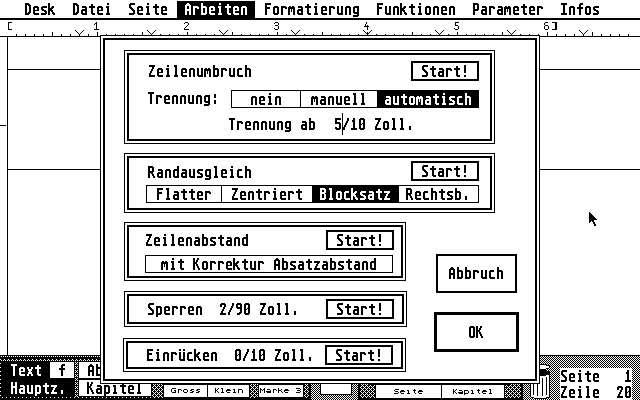
\includegraphics[width=\columnwidth]{img/SNAP4.png}
    \caption{The \textit{Optionen 1...} dialog for text layout}
    \label{fig:text_opts}
\end{figure}

\subsubsection{Accessories \& Tools}

\Signum{} was distributed with a set of additional files that were useful for authoring documents:

\begin{itemize}
    \item Printer \& editor fonts for the character sets \textbf{ANTIKRO}, \textbf{FRAKTUR1}, \textbf{GRAPH1}, \textbf{GRIECH}, \textbf{GROTFE}, \textbf{GROTLT}, \textbf{GROTMIKR}, \textbf{MATHEM}, \textbf{NORMANDE}, and \textbf{PINSEL}.
    \item A set of font editors for the different kinds of printers (\textbf{DCS9N.PRG}, \textbf{DCS24N.PRG} and \textbf{DCS30L.PRG}) as well as a converter from 24-needle printer fonts to laser printer fonts (\textbf{CV24TL30.PRG}).
    \item An \gls{accessory} to capture the current content of the screen to save it as a file that could be loaded into the document (\textbf{SCRCPY.ACC}).
    \item A printer spooler accessory (\textbf{SSP.ACC}) that could improved the printing speed by buffering the output to the actual printer.
    \item A set of printer ''emulators'' that redirected the printer commands to a file (\textbf{PREMUL.PRG}) or to external devices via the serial (\textbf{PEMV24.PRG}), or parallel (\textbf{PEM\_CENT.PRG}) ports.
\end{itemize}

ASH also published a \Signum{} accessory that enabled a right-to-left writing mode, \textbf{SIGREV.ACC}, which proved very useful for scholars that wanted to write Hebrew \cite{stc1988sigrevers}.

\subsection{Fundamentals of File Formats}

A \textit{file format} is a specification that describes how some data is laid out in a \textit{file}, i.e. a sequence of \glspl{byte} that can be saved on a storage device such as a hard disk or flash drive. Most file formats are associated with a file \textit{extension} such as \texttt{*.txt}, \texttt{*.pdf}, \texttt{*.doc} or \texttt{*.png}.

In theory, anyone can specify a file format – either by implementing a software that uses it or by writing a formal specification. In practice, its desirable for software from multiple vendors to use the same, inter-operable file formats.

\subsubsection{Media Types \& Magic Bytes}

To be able to communicate the format of a file without relying on a name or guessing based on the content, the \acrshort{iana} maintains a registry of \glspl{Media Type}\footnote{\url{https://www.iana.org/assignments/media-types/media-types.xhtml}}.

The names listed there are used for downloads and e-mail attachments \cite{rfc6838}. The media types that correspond to the file extensions above are \texttt{text/plain}, \texttt{application/pdf}, \texttt{application/msword}, and \texttt{image/png}.

Some file formats require all \glspl{byte} to be interpreted as characters according to some \gls{encoding}. These are called \textit{text file formats} \cite[§4.2.1]{rfc6838} and should be readable with any plain text editor, for example \textit{Windows Notepad}.

The terms \texttt{ASCII} and \texttt{UTF-8} are used to describe two of the predominant text encoding methods. Formats that include \glspl{byte} that are not encoded as text are usually called \textit{binary file formats}. As the names suggest, files that are stored in a text file format can be edited with a simple text editor, while most binary formats require specialized tools to read or written.

Because file extensions and \acrshort{mime} types are metadata that is not stored in the file itself, most file formats mandate some sort of identifier at the beginning of the file to prevent programs form manipulating a file they were not designed for.

These markers are sometimes called \textit{magic bytes}, presumably because they have no other use than differentiating between formats. For example, a \acrshort{pdf} file always starts with \texttt{\%PDF-} and a \acrshort{png} file with the bytes \fbox{\texttt{89 50 4E 47 0D 0A 1A 0A}}, which contain the string \texttt{PNG}.

\subsubsection{Basic Building Blocks}

This section presents some of the basic building blocks that are used to construct complex file formats. Not all of these apply to the \textit{Signum!} file format, but they should be useful to understand the description in the next section \cite[§1.5]{murray1996eggf}.

\paragraph{Offset \& Format}
There are two aspects that are fundamental to storing a \textit{value} into a file: The first one is the position of that value relative to a reference point or \textit{landmark}. This is called the \textit{offset}. Only two reference points are defined for every file: The \textit{start} and the \textit{end} of the file. %If a format does not require the reference point at the end to start processing, then it's suitable for \textit{streaming}.
The second one is the representation of the data in bytes (or text). This is called the \textit{(binary) format}.

\paragraph{Structures \& Fields}
A \textit{field} is a piece of data that sits at a fixed offset from its reference point. Multiple fields that are stored in sequence starting from a common reference point are collectively called a \textit{struct}.

\paragraph{Arrays \& Streams}
When multiple values of the same kind need to be stored, then they'll usually be stored in sequence. If all values require the same amount of bytes or it's necessary to access one of the elements ''at random'', then every value will be stored at an offset that is a multiple of a known value, the \textit{element length}. This length must be at least as large as the maximum number of bytes that are needed to store one of the values. This whole structure is called an \textit{array}. In some cases, it's useful to store the total length of the array, the element length, or both as a field before the array data to get an array of \textit{variable size}.

Otherwise, when values that would not require the full element length are common or the length is not limited, an element may be stored at next valid offset after the end of the previous one. This is called a \textit{stream} and requires reading all previous elements in order to load a specific one.

\paragraph{Numbers}
On the lowest level of abstraction, all information in a file is stored as numbers. A file is a sequence of \glspl{byte}, each \gls{byte} is made up of 8 \glspl{bit} for a total of 256 different values. In a simple text encoding like ASCII, every character is encoded as one byte value. Sometimes, a byte is subdivided into multiple smaller units, for example 8 units with a value of 0 or 1. This is called a \textit{bitfield}. Sometimes, multiple bytes are grouped to represent a wider range of numbers, e.g. 4 bytes with 32 bits in total, representing 4294967296 distinct values.

\paragraph{Indirect Values}
When the same value is needed multiple times in a file format, it may be useful to store it only once and use a \textit{reference} to that location wherever it is used. One approach to do that is to use the \textit{offset} of the actual value. The other approach is to put these values in an array or stream that is stored somewhere else in the file and use the position in that sequence (the \textit{index}) to represent the value.

\paragraph{Tags}
It's also possible for the structure of the file to depend on the data that is stored. In a format like \LaTeX, a \texttt{\%} sign indicates a comment and \texttt{\textbackslash} indicates a control sequence. In languages like HTML or XML, a \texttt{<} sign indicates a \textit{named tag} and a \texttt{\&} indicates a \textit{named entity}\footnote{Pre-defined text, usually used for writing single characters that are not part of ASCII, e.g. \texttt{euro} for the \euro{} sign}. In other formats, a character code of $0$ is used to mark the end of a string (stream of characters) because it will not appear in any text value. In text formats, it's common for tags to have a matching end tag. A \LaTeX{} comment is terminated by a newline, a HTML named tag is terminated by a \texttt{>} sign and some named tags like \texttt{<a>} require a corresponding closing tag \texttt{</a>}.

\paragraph{Chunks}
Instead of having a dedicated start and end tag, you can also combine a marker with a run-length specifier to specify the bounds of a \textit{chunk}. An early example of a file format using this is the  \acrfull{iff} which uses \acrfullpl{four-cc} to identify file formats and different kinds of parts of the file.

\subsection{Anatomy of a word document}

The Signum!2 document file format uses the file extension \textbf{SDO} and the magic \glspl{byte} are \texttt{sdoc0001}. There is no \textit{Media Type} registered with the IANA for the format.

The general layout of the file format is very similar to and likely inspired by the \acrshort{iff}. The leading \texttt{sdoc} is one example of a \acrshort{four-cc}. Both the \acrshort{iff} \texttt{FORM} format and the \Signum{} file format use a sequence of chunks, saved as pairs of one \acrshort{four-cc} and a 32-bit length specifier followed by a block of data of that length. While \acrshort{iff} files generally use the same chunk type multiple times \cite{amigaos:wordiff}, that is not the case for Signum files. The following subsections present the chunks that it uses in the order that they generally appear in.

One important aspect of this file format is that it is forward- and backward-compatible, that is, newer versions of the software can use files created by older versions and older versions can edit files created by newer versions to some extent without destroying information.

\subsubsection{Header (\texttt{0001})}
\label{sec:sdoc_0001}

The name \textbf{0001} was probably intended to specify the version. This chunk does not contain much data. It does contain information on when the document was created and when it was last saved.

\subsubsection{Character Sets (\texttt{cset})}
\label{sec:sdoc_cset}

The first important section of a Signum! document uses the \textbf{cset} identifier. This section contains an \textit{array} of 8 names with up to 9 characters each. It corresponds to the list of \textit{charsets} that are selected for the document.

Note that the length of the names roughly corresponds to the 8 \gls{byte} limit on file names on the ATARI ST (cf. section 3.1 of \cite{guerin2014filesystem}).

The rest of the file format uses the numbers $0$ through $6$ to represent theses characters sets, so this section is used as a \textit{lookup table} to select the relevant one for a number. In \autoref{fig:cset-dialog}, \textbf{ANTIKRO} would be number $0$, \textbf{NORMANDE} would be number $1$ and \textbf{MATHEM} would be number $2$.

\subsubsection{System Parameters (\texttt{sysp})}
\label{sec:sdoc_sysp}

The next section bears the identifier \textbf{sysp}. At its core, the \Signum{} file format is more of a graphics format than a text format. The parameters correspond to the \textit{Std. Seitenformat} i.e. standard page formatting options in the user interface and are used to set the initial parameters of new pages.

The section also contains additional global configuration such as the settings for automatic page numbering.

\subsubsection{Page Buffer (\texttt{pbuf})}
\label{sec:sdoc_pbuf}

This section (marked \textbf{pbuf}) contains a table with parameters for each page in the document. It starts with the number of pages and the number of \glspl{byte} used for every entry.

Each entry contains an internal index, the logical page number i.e. position within the current document and the physical page number i.e. the position in all documents that make up the final text. It also contains the length of the header and footer as well as the position of the left and right print margin in terms of horizontal coordinates.

\subsubsection{Text Buffer (\texttt{tebu})}
\label{sec:sdoc_tebu}

\begin{figure}[ht]
    \centering
    \begin{Verbatim}[fontsize=\small]
00520c00 40490090 40490005 40490005 .R..@I..@I..@I..
402e0005 4044000b 4049000a 40450005 @...@D..@I..@E..
40520010 40450009 40490009 40430005 @R..@E..@I..@C..
4048000a 4053000b 404b0008 404c000a @H..@S..@K..@L..
407b0008 4053000b 40540008 40450009 @{..@S..@T..@E..
40520009 00120076 0c000045 00979269 @R.....v...E...i
886e9065 8e73a464 90658e72 a2629065 .n.e.s.d.e.r.b.e
8e649065 8e759074 8c658e6e 90738e74 .d.e.u.t.e.n.s.t
8c658e6e a65a9265 8e759067 906e9069 .e.n.Z.e.u.g.n.i
88738e73 8e65a466 8c409072 a2649069 .s.s.e.f.@.r.d.i%
\end{Verbatim}
    \caption{Portion of the text buffer of a document as displayed in a hex-editor. The actual text is supposed to be \foreigntextquote{german}{\underline{III. DIE REICHSKLÖSTER}} and \foreigntextquote{german}{Eines der bedeutensten Zeugnisse für die {[\dots]}} \label{fig:sdo-hexdump}}
\end{figure}

This section uses \textbf{tebu} as its identifier. It is stored as a sequence of chunks that represent the start of a page, the end of a page or a line of characters within a page. Empty lines are not stored. Instead, every line with content starts with a number that specifies how many empty lines were skipped.

The same principle applies within a line: The line is a sequence of character tags that contain the distance from the previous character position, the number of the character set that was used, the number of the character itself and some individual bits that specify which font variants (\ref{sec:font-variants}) were used.

\subsubsection{Hardcopies \& Images (\texttt{hcim})}
\label{sec:sdoc_hcim}

This section is indicated by the \acrshort{four-cc} \textbf{hcim} and contains a sequence of images (hardcopies) that can be used within the document as well as a cross-reference table that defines where parts of the images are actually used.

Because the first version of Signum! did not support images, it's noteworthy that all information related to them is stored in this separate section. This way, an older version of signum can be used to make small changes to the text while keeping this section and thus all images and their position unchanged.

The section starts with a 16 \gls{byte} long header that contains the size in \glspl{byte} of the cross-reference (``site'') table, the number of images and the number of sites.

The header is followed by the site table, which consists of a sequence of 32 \gls{byte} entries that store information like the page, position, height, width and selected area of the original image.

Finally, there is the table of images, which are stored with a filename and encoded according to the \textit{bimc} image file format.

\subsubsection{Unknown sections (\texttt{pl01} \& \texttt{syp2})}
The function of these two chunks is unknown.

\subsection{The \textit{bimc} Image format}

\newcommand{\fboxinclude}[1]{\fbox{\includegraphics[width=0.08\textwidth]{#1}}}
\newcommand{\chk}[1]{\fbox{\makebox(20,20){#1}}}
\newcommand{\chdots}{\makebox(28,26){$\dots$}}
\newcommand{\cvdots}{\makebox(28,26){$\vdots$}}
\newcommand{\cmid}{\makebox(28,26){}}

The \textbf{bimc} file format, specifically version 2 according to the magic \glspl{byte} \textbf{bimc0002}, is a compression scheme for black-and-white images that was used by multiple \gls{ASH} products\footnote{\url{https://www.stcarchiv.de/stm1991/12/piccolo}}.

In the past, there was barely any information publicly available\footnote{\url{https://temlib.org/AtariForumWiki/index.php/Signum!_file_format}} on the details of this format. This is probably due to the fact that \acrshort{ash} products are proprietary and mostly sold to a german audience.

Based on the \textit{68K decompression code} mentioned on that page, I was able to reverse engineer and document the actual compression method.

\subsubsection{Introduction to the compression method}

The \Signum{} handbook \cite[p.~26]{schmerbeck1998signum} explains that a \gls{hardcopy} has the size of an ATARI ST screen i.e. a width of 640 pixels and a height of 400 pixels (\textit{ST-High}). All \textbf{bimc} images that I could find had this size.

\begin{figure}[h]
    \centering
    \chk{$0$} \chk{$1$} \chk{$2$} \chdots \chk{$37$} \chk{$38$} \chk{$39$}\\
    \chk{$40$} \chk{$41$} \chk{$42$} \chdots \chk{$77$} \chk{$78$} \chk{$79$}\\
    \cvdots \cvdots \cvdots \cmid \cvdots \cvdots \cvdots\\
    \chk{$920$} \chk{$921$} \chk{$922$} \chdots \chk{$957$} \chk{$958$} \chk{$959$}\\
    \chk{$960$} \chk{$961$} \chk{$962$} \chdots \chk{$997$} \chk{$998$} \chk{$999$}
    \caption{Position and numbering of chunks in the \textbf{bimc} compression scheme. Every picture has 25 rows and every row has 40 chunks.}
    \label{fig:bimc_chunk_layout}
\end{figure}

The image is partitioned into chunks of 16x16 pixels from left to right, top to bottom i.e. normal English reading order. For the default image size, that is $40 \times 25 = 1000$ chunks in total. Each chunk is further subdivided into four 8x8 sub-chunks: top-left ($A$), top-right ($B$), bottom-left ($C$), and bottom-right ($D$).

\begin{figure}[h]
    \centering
    \chk{$A$} \chk{$B$} \\[1mm]
    \chk{$C$} \chk{$D$}
    \caption{Structure of a chunk in the \textbf{bimc} compression scheme. Each chunk is made up of four $8 \times 8$ pixel sub-chunks.}
    \label{fig:bimc_subchunk_layout}
\end{figure}

It is saved as two sequences: One sequence of bits that we'll call the \textit{control stream} and one sequence of \glspl{byte} that we'll call the \textit{data stream}. In the original, uncompressed image, black is stored as $1$ (\textit{ink}) and white is stored as $0$ (\textit{no ink}).

\paragraph{Concept}
The basic idea of the compression algorithm is only serializing rows-of-chunks, chunks, sub-chunks and rows of pixels in sub-chunks that are non-zero. Additionally, the built-in support for top-to-bottom repetition can switch a lot of the bits to zero if most of the image or most of a chunk uses a plain or checkered background. That last one is useful because a checkered background was commonly used for shades of gray on screens that only supported black and white \cite{toshyp:VDIpatterns}.

\newcommand{\ws}{\square}
\newcommand{\bs}{\blacksquare}
\newcommand{\wbyte}{$\ws\ws\ws\ws\ws\ws\ws\ws$}
\newcommand{\bbyte}{$\bs\bs\bs\bs\bs\bs\bs\bs$}
\newcommand{\wbbyte}{$\ws\bs\ws\bs\ws\bs\ws\bs$}
\newcommand{\bwbyte}{$\bs\ws\bs\ws\bs\ws\bs\ws$}

\paragraph{Note}
The following algorithm uses an operation called \textbf{XOR}. This is short for \textit{Exclusive-Or} because it's identical to using a black pixel if and only if pixels at the same position differ. For example, $\ws\ws\bs\bs \text{ XOR } \ws\bs\bs\ws$ equals $\ws\bs\ws\bs$. Another interpretation is to flip every color (bit) in one operand that is black (set) in the other. Note that the order of the operands does not matter, only that they have the same length.

\subsubsection{Decoding algorithm}

The algorithm to decode and encode images is has two components: The \textit{outer loop} that iterates over the full image and calls a \textit{chunk decoding} algorithm that decodes a single chunk. Decoding requires knowing the width and height of the final image as well as two XOR bytes. These values are provided in the file header.

\paragraph{Outer loop}

\begin{enumerate}
    \item Start with an all-zero (white) image of $600 \times 420$ pixels.
    \item Prepare a 32 \gls{byte} buffer to decode a chunk.
    \item Look at the first row of chunks.
    \item Take one bit from the control stream. If that bit is $0$, skip to step 9.
    \item Otherwise, Look at the first chunk in the current row.
    \item Take one bit from the control stream. If that bit is $0$, skip to step 8.
    \item Decode the chunk using the \textit{chunk decoding} algorithm. Copy the sixteen pairs of \glspl{byte} that represent the sixteen rows of pixels from the buffer to the final image.
    \item Check whether there's another chunk in the same row. If so, move to the next chunk and continue with step 6.
    \item Check whether there's another row in the picture. If so, move to the next row and continue with step 4.
    \item Take the first XOR byte from the header and combine that with every even row of pixels in every sub-chunk.
    \item Finally, take the second XOR byte from the header and combine that with every off row of pixels in every sub-chunk.
\end{enumerate}

\begin{figure}[h]
    \centering
    \fboxinclude{img/bimc-lg/bimc-ex-0-lg.png}%
    \fboxinclude{img/bimc-lg/bimc-ex-1-lg.png}%
    \fboxinclude{img/bimc-lg/bimc-ex-2-lg.png}%
    \fboxinclude{img/bimc-lg/bimc-ex-3-lg.png}%
    \fboxinclude{img/bimc-lg/bimc-ex-4-lg.png}\\[1mm]%
    \fboxinclude{img/bimc-lg/bimc-ex-5-lg.png}%
    \fboxinclude{img/bimc-lg/bimc-ex-6-lg.png}%
    \fboxinclude{img/bimc-lg/bimc-ex-7-lg.png}%
    \fboxinclude{img/bimc-lg/bimc-ex-8-lg.png}%
    \fboxinclude{img/bimc-lg/bimc-ex-9-lg.png}
    \caption{Example of BIMC compressed data. Instead of 32 \glspl{byte} for all 256 pixels, we need only 13 \glspl{byte}. One for every sub-chunk with black pixels and one for every row in a sub-chunk with black pixels}
    \label{fig:bimc_subchunk_data}
\end{figure}

\paragraph{Chunk decoding}
%Recall that every sub-chunk made up of 8 rows that are 8 pixels wide. Starting a $0$, we call rows $0, 2, 4$ and $6$ \textit{even} and rows $1, 3, 5$ and $7$ \textit{odd}.

\begin{enumerate}
    \item Take 2 bits from the control stream. This is the compression mode.
    \item If the bits are $11$ load the next 32 \glspl{byte} from the data stream into the buffer and skip the steps 3 to 7.
    \item Otherwise, take another 4 bits out of the control stream. This is the sub-chunk mask.
    \item If the first bit is set, take one \gls{byte} from the data stream and look at its bits. Every bit corresponds to one of the positions $0, 2, 4, 6, 8, 10, 12, 14$ in the buffer. If it is set, take one \gls{byte} from the data stream and put it in that position. This is the top-left sub-chunk $A$.
    \item Do the same for the second bit of the sub-chunk mask and positions $1, 3, 5, 7, 9, 11, 13, 15$ (top right sub-chunk $B$), the third bit of the sub-chunk mask and positions $16, 18, 20, 22, 24, 26, 28, 30$ (bottom-left sub-chunk $C$), and the fourth bit of the sub-chunk mask and positions $17, 19, 21, 23, 25, 27, 29, 31$. (bottom-right sub-chunk $D$).
    \item Now, recall the compression mode. If the bits are $01$, take \glspl{byte} $0$ and $1$ from the buffer and XOR them with bytes $2$ and $3$. Take the resulting two bytes and XOR them with bytes $4$ and $5$. Repeat that for the complete buffer.
    \item Otherwise, if the compression mode was $10$, take the first four \glspl{byte} ($0$ to $3$ i.e two rows of pixels) and XOR them with \glspl{byte} $4$ through $7$. Take the resulting 4 bytes and XOR them with the next four. Repeat that for the rest of the buffer.
\end{enumerate}

Done!

\begin{figure}[h]
    \centering
    \fboxinclude{img/bimc-lg/bimc-ex-9-lg.png}$\to$%
    \fboxinclude{img/bimc-lg/bimc-ex-10-lg.png}$\to$%
    \fboxinclude{img/bimc-lg/bimc-ex-11-lg.png}$\to$%
    \fboxinclude{img/bimc-lg/bimc-ex-12-lg.png}\\[2mm]$\to$%
    \fboxinclude{img/bimc-lg/bimc-ex-13-lg.png}$\to$%
    \fboxinclude{img/bimc-lg/bimc-ex-14-lg.png}$\to$%
    \fboxinclude{img/bimc-lg/bimc-ex-15-lg.png}$\to$%
    \fboxinclude{img/bimc-lg/bimc-ex-16-lg.png}
    \caption{Example of the final step of decoding a chunk that was compressed with strategy 2. \label{fig:bimc_chunk_xor}}
\end{figure}

%\subsubsection{Encoding algorithm}
%
%The encoding algorithm is the same procedure just in reverse. The main challenge in writing the encoder is to choose a good compression mode for each chunk and good final XOR bytes without taking too much time analyzing the uncompressed image. The following algorithm proposes methods to achieve this but actual implementations may choose a different approach. We call a row, chunk, sub-chunk or row of a sub-chunk \textit{non-white} if at least one of its pixels is black.
%
%\paragraph{Outer loop}
%
%\begin{enumerate}
%    \item For every even row in every sub-chunk, find the pattern
%    that is most common. Let's call that pattern $X_A$. Do the same for every odd row in every odd sub-chunk and call that $X_B$. For an image that is predominantly white, both will be \wbyte. For an image that is predominantly black, both will be \bbyte. For an image that is predominantly checkered, one might be \bwbyte~while the other is \wbbyte.
%    \item Now, for every even row in every sub-chunk, flip every pixel that is black in $X_A$. Do the same for every odd row in every sub-chunk but with $X_B$. This has the effect that the most common row is \wbyte~now.
%    \item Now, start on the first row of chunks
%    \item If the complete row is white, write a $0$ to the control stream and skip to step 9
%    \item Otherwise, look at the first chunk in the row
%    \item If the complete chunk is white, write a $0$ to the control stream and skip to step 8
%    \item Encode the chunk using the \textit{chunk encoding} algorithm.
%    \item Check whether there's another chunk in the same row. If so, move to the next chunk and continue with step 6.
%    \item Check whether there's another row in the picture. If so, move to the next row and continue with step 4.
%    \item Save the file and store $X_A$ and $X_B$ in its header.
%\end{enumerate}
%
%\paragraph{Chunk encoding}
%
%\begin{enumerate}
%    \item Count the number of sub-chunks that are not completely white plus the total number of non-white rows in these sub-chunks. We'll call that $c_0$.
%    \item Then, count the number of sub-chunks and rows that are non-white when every row (except the first) is XOR-ed with the row directly above. We'll call that $c_1$.
%    \item Then, count the number of sub-chunks and rows that are non-white when every row (except the first two) is XOR-ed with the row two above them. We'll call that $c_2$.
%    \item Finally, set $c_3$ to $32$. Each value $c_x$ represents the number of bytes that are written for one of the compression modes $x \in {0, 1, 2, 3}$.
%    \item Now, choose the compression mode $x$ with the minimal value for $c_x$. If that minimum is $32$, choose mode $3$. Write the compression mode to the control stream as a 2-bit binary number.
%    \item If the compression mode is $3$, write the complete buffer to the data stream and skip the last two steps.
%    \item Otherwise, apply the XOR-operations for modes $1$ and $2$.
%    \item Then, for every sub-chunk ($A,B,C,D$), write $0$ to the control stream if the sub-chunk is completely white. Otherwise, write $1$ to the control stream and one \gls{byte} to the data stream where each indicates whether the corresponding row is non-white. Then, write those non-white row in the sub-chunk to the data stream.
%\end{enumerate}
%
%Done!